\documentclass{standalone}
\usepackage{tikz}
\usetikzlibrary{patterns}
\usetikzlibrary{positioning}
\usetikzlibrary{patterns, positioning}
\usetikzlibrary{shapes.misc}
\usepackage[outline]{contour}
\contourlength{1.5pt} 
\usepackage[sfdefault]{ClearSans}

\begin{document}
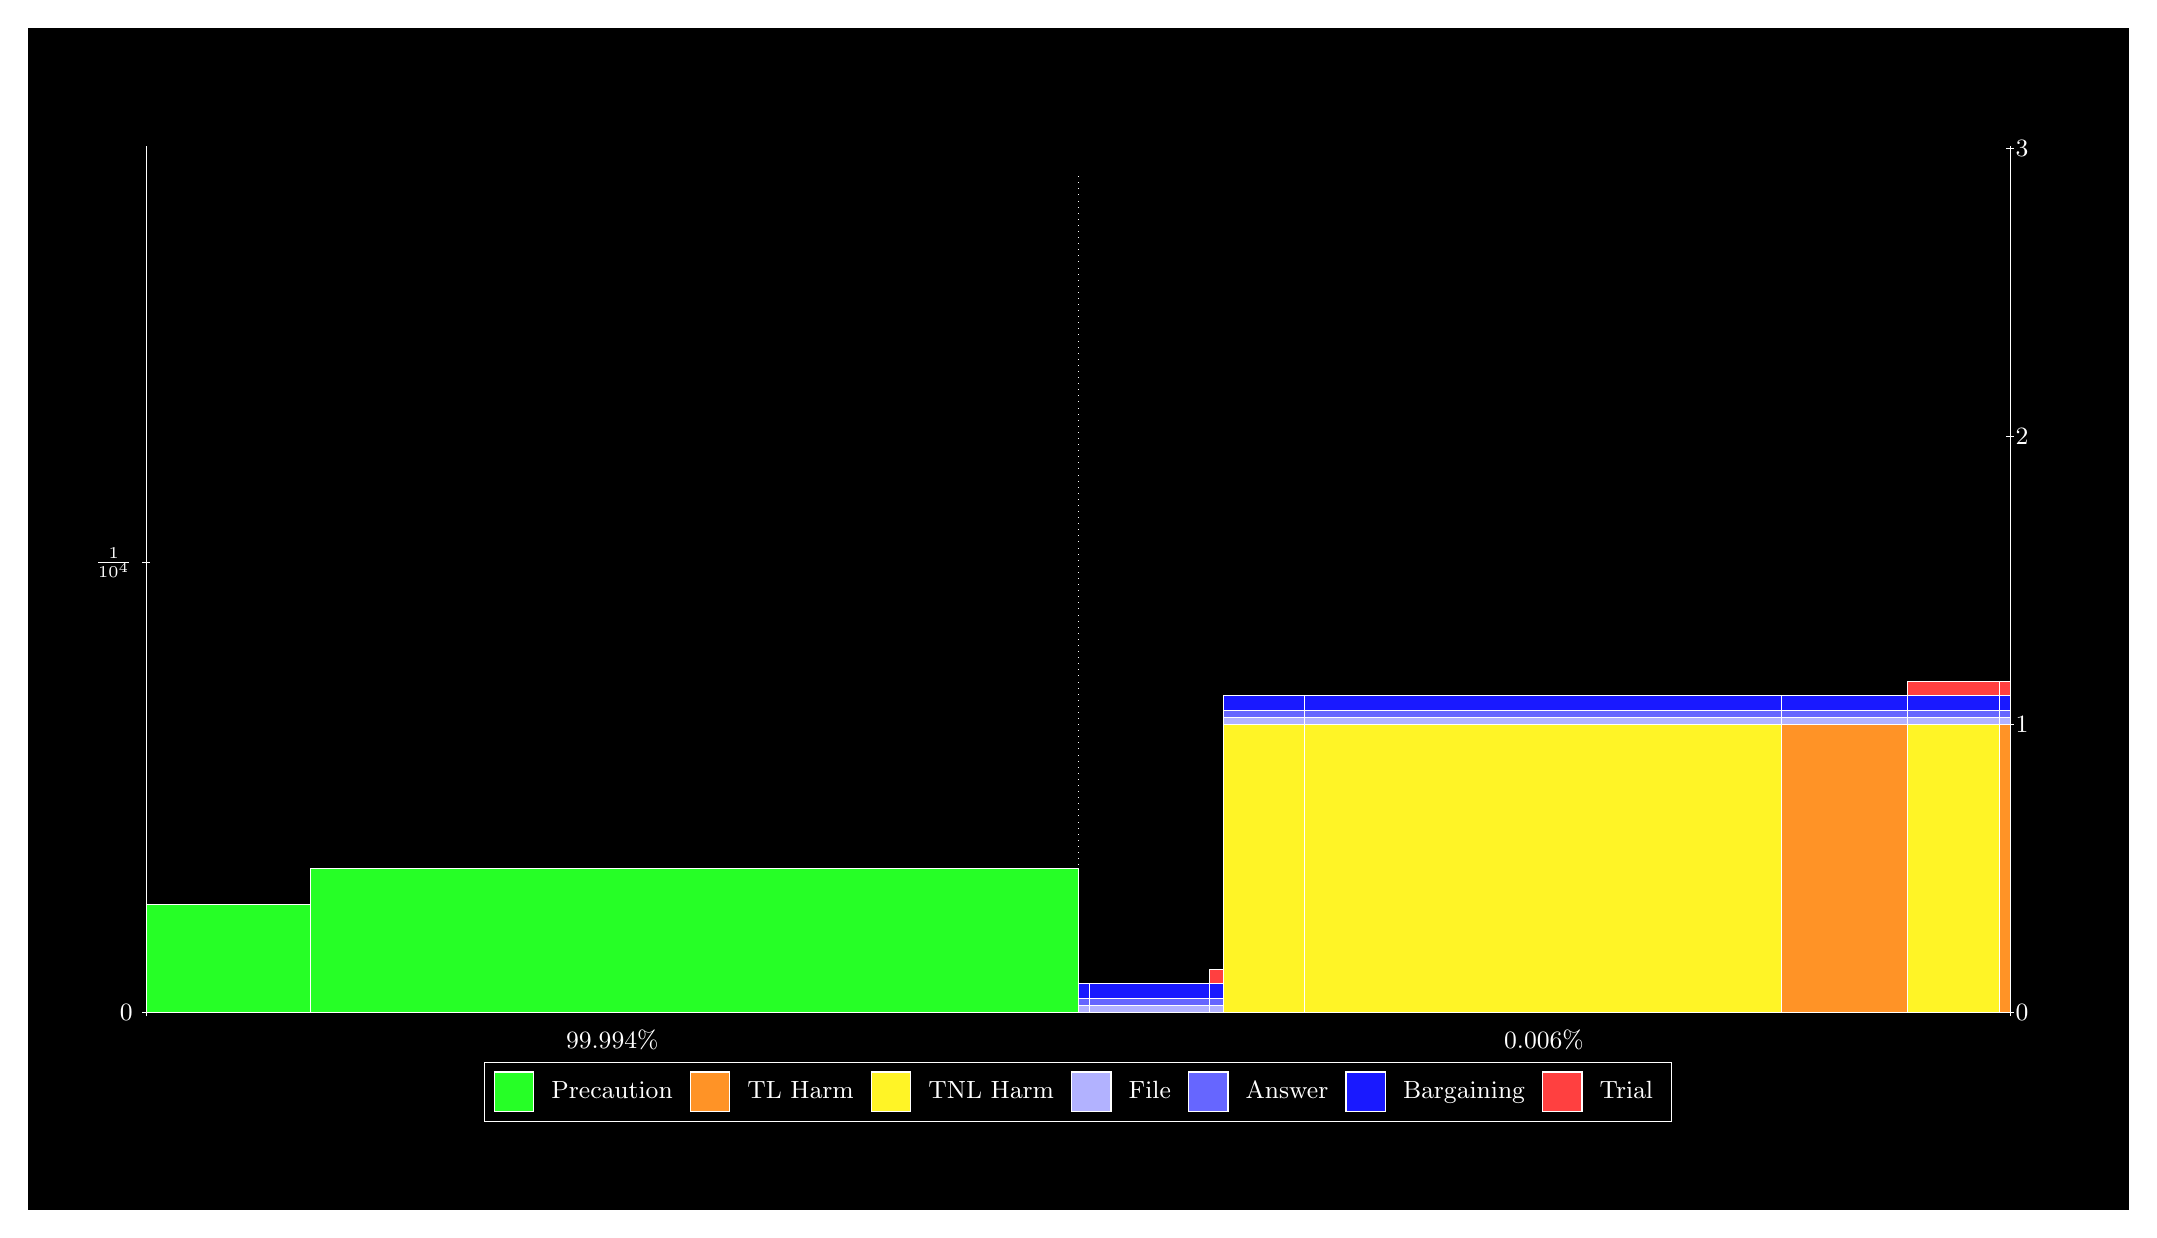
\begin{tikzpicture}
\draw[fill=black] (0,0) rectangle (26.667,15);
\draw[fill=green!85,draw=white,very thin] (1.5,2.5) rectangle (3.585,3.8714);
\draw[fill=green!85,draw=white,very thin] (3.585,2.5) rectangle (13.333,4.3285);
\draw[fill=green!85,draw=white,very thin] (13.333,2.5) rectangle (13.473,2.5001);
\draw[fill=blue!30,draw=white,very thin] (13.333,2.5001) rectangle (13.473,2.5915);
\draw[fill=blue!60,draw=white,very thin] (13.333,2.5915) rectangle (13.473,2.683);
\draw[fill=blue!90,draw=white,very thin] (13.333,2.683) rectangle (13.473,2.8658);
\draw[fill=green!85,draw=white,very thin] (13.473,2.5) rectangle (14.996,2.5001);
\draw[fill=blue!30,draw=white,very thin] (13.473,2.5001) rectangle (14.996,2.5916);
\draw[fill=blue!60,draw=white,very thin] (13.473,2.5916) rectangle (14.996,2.683);
\draw[fill=blue!90,draw=white,very thin] (13.473,2.683) rectangle (14.996,2.8659);
\draw[fill=green!85,draw=white,very thin] (14.996,2.5) rectangle (15.182,2.5001);
\draw[fill=blue!30,draw=white,very thin] (14.996,2.5001) rectangle (15.182,2.5915);
\draw[fill=blue!60,draw=white,very thin] (14.996,2.5915) rectangle (15.182,2.683);
\draw[fill=blue!90,draw=white,very thin] (14.996,2.683) rectangle (15.182,2.8658);
\draw[fill=red!75,draw=white,very thin] (14.996,2.8658) rectangle (15.182,3.0487);
\draw[fill=green!85,draw=white,very thin] (15.182,2.5) rectangle (16.204,2.5001);
\draw[fill=yellow!85,draw=white,very thin] (15.182,2.5001) rectangle (16.204,6.1576);
\draw[fill=blue!30,draw=white,very thin] (15.182,6.1576) rectangle (16.204,6.249);
\draw[fill=blue!60,draw=white,very thin] (15.182,6.249) rectangle (16.204,6.3405);
\draw[fill=blue!90,draw=white,very thin] (15.182,6.3405) rectangle (16.204,6.5234);
\draw[fill=green!85,draw=white,very thin] (16.204,2.5) rectangle (16.211,2.5001);
\draw[fill=orange!85,draw=white,very thin] (16.204,2.5001) rectangle (16.211,6.1576);
\draw[fill=blue!30,draw=white,very thin] (16.204,6.1576) rectangle (16.211,6.249);
\draw[fill=blue!60,draw=white,very thin] (16.204,6.249) rectangle (16.211,6.3405);
\draw[fill=blue!90,draw=white,very thin] (16.204,6.3405) rectangle (16.211,6.5234);
\draw[fill=green!85,draw=white,very thin] (16.211,2.5) rectangle (22.263,2.5001);
\draw[fill=yellow!85,draw=white,very thin] (16.211,2.5001) rectangle (22.263,6.1576);
\draw[fill=blue!30,draw=white,very thin] (16.211,6.1576) rectangle (22.263,6.2491);
\draw[fill=blue!60,draw=white,very thin] (16.211,6.2491) rectangle (22.263,6.3405);
\draw[fill=blue!90,draw=white,very thin] (16.211,6.3405) rectangle (22.263,6.5234);
\draw[fill=green!85,draw=white,very thin] (22.263,2.5) rectangle (23.86,2.5001);
\draw[fill=orange!85,draw=white,very thin] (22.263,2.5001) rectangle (23.86,6.1576);
\draw[fill=blue!30,draw=white,very thin] (22.263,6.1576) rectangle (23.86,6.2491);
\draw[fill=blue!60,draw=white,very thin] (22.263,6.2491) rectangle (23.86,6.3405);
\draw[fill=blue!90,draw=white,very thin] (22.263,6.3405) rectangle (23.86,6.5234);
\draw[fill=green!85,draw=white,very thin] (23.86,2.5) rectangle (25.027,2.5001);
\draw[fill=yellow!85,draw=white,very thin] (23.86,2.5001) rectangle (25.027,6.1576);
\draw[fill=blue!30,draw=white,very thin] (23.86,6.1576) rectangle (25.027,6.249);
\draw[fill=blue!60,draw=white,very thin] (23.86,6.249) rectangle (25.027,6.3405);
\draw[fill=blue!90,draw=white,very thin] (23.86,6.3405) rectangle (25.027,6.5234);
\draw[fill=red!75,draw=white,very thin] (23.86,6.5234) rectangle (25.027,6.7062);
\draw[fill=green!85,draw=white,very thin] (25.027,2.5) rectangle (25.167,2.5001);
\draw[fill=orange!85,draw=white,very thin] (25.027,2.5001) rectangle (25.167,6.1576);
\draw[fill=blue!30,draw=white,very thin] (25.027,6.1576) rectangle (25.167,6.249);
\draw[fill=blue!60,draw=white,very thin] (25.027,6.249) rectangle (25.167,6.3405);
\draw[fill=blue!90,draw=white,very thin] (25.027,6.3405) rectangle (25.167,6.5234);
\draw[fill=red!75,draw=white,very thin] (25.027,6.5234) rectangle (25.167,6.7062);
\draw[white,very thin] (1.5,2.5) -- (1.5,13.5);
\draw[white,very thin] (1.45,2.5) -- (1.55,2.5);
\node[font=\small,text=white, anchor=east] at (1.45, 2.5) {0};
\draw[white,very thin] (1.45,8.214) -- (1.55,8.214);
\node[font=\small,text=white, anchor=east] at (1.45, 8.214) {$\frac{1}{10^{4}}$};

\draw[white,dotted,very thin] (13.333,2.83) -- (13.333,13.17);
\draw[white,very thin] (25.167,2.5) -- (25.167,13.5);
\draw[white,very thin] (25.117,2.5) -- (25.217,2.5);
\node[font=\small,text=white, anchor=west] at (25.117, 2.5) {0};
\draw[white,very thin] (25.117,6.1575) -- (25.217,6.1575);
\node[font=\small,text=white, anchor=west] at (25.117, 6.1575) {1};
\draw[white,very thin] (25.117,9.815) -- (25.217,9.815);
\node[font=\small,text=white, anchor=west] at (25.117, 9.815) {2};
\draw[white,very thin] (25.117,13.473) -- (25.217,13.473);
\node[font=\small,text=white, anchor=west] at (25.117, 13.473) {3};

\draw[white,very thin] (1.5,2.5) -- (25.167,2.5);
\draw[white,very thin] (1.5,2.45) -- (1.5,2.55);
\node[font=\small,text=white, anchor=north] at (1.5, 2.45) {};
\draw[white,very thin] (25.167,2.45) -- (25.167,2.55);
\node[font=\small,text=white, anchor=north] at (25.167, 2.45) {};

\node[font=\small,text=white,anchor=south] at (7.4167, 1.9) {99.994\%};
\node[font=\small,text=white,anchor=south] at (19.25, 1.9) {0.006\%};
\draw (13.3333,2.5) node (B) {};
\begin{scope}[align=center]
\matrix[scale=0.5,draw=white,below=0.5cm of B,nodes={draw},column sep=0.1cm]{
\node[rectangle,draw,minimum width=0.5cm,minimum height=0.5cm,fill=green!85]{}; & \node[draw=none,font=\small,text=white]{Precaution}; &
\node[rectangle,draw,minimum width=0.5cm,minimum height=0.5cm,fill=orange!85]{}; & \node[draw=none,font=\small,text=white]{TL Harm}; &
\node[rectangle,draw,minimum width=0.5cm,minimum height=0.5cm,fill=yellow!85]{}; & \node[draw=none,font=\small,text=white]{TNL Harm}; &
\node[rectangle,draw,minimum width=0.5cm,minimum height=0.5cm,fill=blue!30]{}; & \node[draw=none,font=\small,text=white]{File}; &
\node[rectangle,draw,minimum width=0.5cm,minimum height=0.5cm,fill=blue!60]{}; & \node[draw=none,font=\small,text=white]{Answer}; &
\node[rectangle,draw,minimum width=0.5cm,minimum height=0.5cm,fill=blue!90]{}; & \node[draw=none,font=\small,text=white]{Bargaining}; &
\node[rectangle,draw,minimum width=0.5cm,minimum height=0.5cm,fill=red!75]{}; & \node[draw=none,font=\small,text=white]{Trial}; \\\\
};\end{scope}

\end{tikzpicture}
\end{document}